%% implemen.tex
\chapter{Implementierung}
\label{ch:Implementierung}
%% ==============================
Dieses Kapitel befasst sich mit der Implementierung der Algorithmen aus Kapitel \ref{ch:Grundlagen}. Zuerst werden jeweils die Ein- und Ausgaben der verschiedenen Nodes, deren Nutzen und Funktionsweise erklärt. 
Danach werden die einzelnen Schritte der Implementierung des NodeDialogs und NodeModels erläutert. Falls eine Implementierung eines Views vorhanden ist, wird diese auch präsentiert.
%% ==============================
\section{PreferenceCreator Node}
\label{ch:Implementierung:sec:prefCreatorNode}
%% ==============================
\begin{figure}[H]
	\centering
	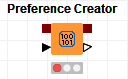
\includegraphics[width=0.23\textwidth]{prefCreatorLogo.png}
	\caption{PreferenceCreator Node}
	\label{img:prefCreatorLogo}
\end{figure} 

In Figur \ref{img:prefCreatorLogo} ist der PreferenceCreator Node zu sehen. Dieser nimmt als Eingabe ein DatabasePortObject und einen BufferedDataTable an. Das DatabasePortObject enthält den Typ der Datenbankverbindung, einen SQL-Query und die entsprechende Verbindung mit Datenbank-URL und JDBC Treiber. Zusätzlich enthält das Objekt auch einen Usernamen und das dazugehörige Passwort, falls dies für die Datenbank Authentifizierung notwendig ist. Mit Hilfe des Querys und der Verbindung können Datensätze abgerufen werden und für den Algorithmus verwendet werden. 
In Abbildung \ref{img:prefCreatorDBConnection} ist einer dieser Objekte mit allen eingegeben Daten zu sehen, wohingegen Abbildung \ref{img:prefCreatorDataTable} einem Teil der Datensätzen des BufferedDataTables entspricht. Dieser BufferedDataTable wird für den NodeDialog benötigt, um alle Dimensionen dieser Tabelle in einer Auswahlbox anzuzeigen, da im NodeDialog die Datensätze nicht mit der Datenbankverbindung abgerufen werden können. Es ist notwendig, dass mit dem Query des DatabasePortObjects der gleiche BufferedDataTable entsteht, der als Eingabe in den Node kommt, da sonst mit falschen Daten weitergearbeitet wird. Deshalb wird in der $configure$ Methode des NodeModels geprüft, ob das DatabasePortObject den gleichen BufferedDataTable zurück liefert wie der als Eingabe in diesen Node kommende BufferedDataTable. Falls dieser Test fehlschlägt, kann der Node nicht ausgeführt werden. 

\begin{figure}[H]
	\centering
	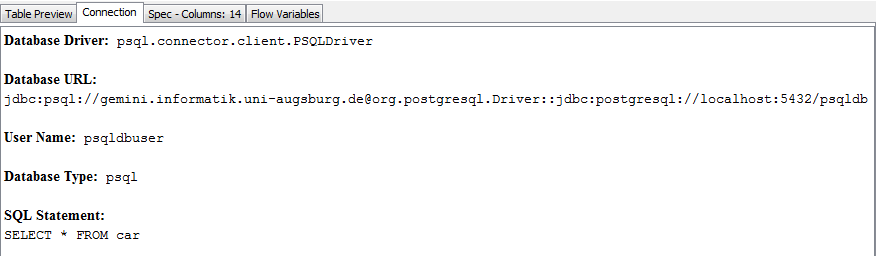
\includegraphics[width=0.85\textwidth]{prefCreatorDBConnection.png}
	\caption{DataBaseConnection Inport des PreferenceCreator Nodes}
	\label{img:prefCreatorDBConnection}
\end{figure}

\begin{figure}[H]
	\centering
	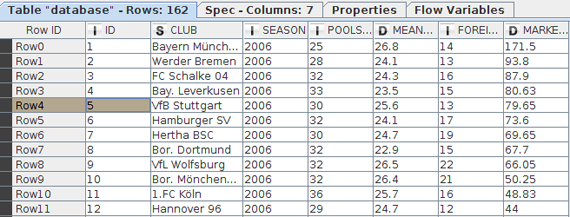
\includegraphics[width=1.0\textwidth]{prefCreatorDataTable.png}
	\caption{BufferedDataTable Inport des PreferenceCreator Nodes}
	\label{img:prefCreatorDataTable}
\end{figure}

Bei der Ausführung des Nodes werden zwei SQL-Queries erzeugt. Der Score-Query und der Preference-Query. Der Score-Query bewertet jeden Datensatz anhand der Präferenzen des Users, die im NodeDialog eingegeben werden und der Preference-Query entspricht einem Preference-SQL Query (siehe Kapitel \ref{ch:Forschungsstand:sec:prefSQL}) basierend auf den selben Präferenzen. 

Einer der Ausgaben des Nodes entspricht dem selben DataBasePortObject, welches als Eingabe in den Node kommt. Diese Ausgabe wird von nachfolgenden Nodes benutzt, um sich mit der Datenbank zu verbinden und dadurch ein Zugriff auf die originalen Daten möglich ist. Die meisten nachfolgende Nodes benutzen sowohl den Score-Query als auch den ursprünglichen Query, der als  Zusatzinformation für das DatabasePortObject enthalten ist. Der Grund dafür ist, dass die meisten Nodes dieser Arbeit sowohl die bewerteten Datensätze (Datensätze, die durch den Score-Query entstehen), als auch den Originaldatensatz benötigen. Um beides zu ermöglichen, werden der Score-Query, der Preference-Query und weitere Informationen, die später noch genannt werden, als versteckte Flowvariablen an folgende Nodes weitergegeben. Nachfolgende Nodes sind hierbei alle Nodes, die im vorhergehenden Datenfluss einen PreferenceCreator Node besitzen. Diese müssen nicht zwingend direkte Nachfolger des PreferenceCreator Nodes sein, sondern können auch Enkelkinder sein.

Wie schon erwähnt benutzen die meisten Nodes den Score-Query mit den bewerteten Datensätzen und den ursprünglichen Query. Der Preference-Query wird bisher nur von dem PreferenceSQLExtract (Abschnitt \ref{ch:Implementierung:sec:prefSQLExtract}) und dem PreferenceSQL Node (Abschnitt \ref{ch:Implementierung:sec:prefSQL}) benutzt. 

Die zweite Ausgabe stellt die Scoretabelle da, einen BufferedDataTable der durch eine Abfrage des Score-Queries an die Datenbankverbindung entsteht. Diese Ausgabe ist ein optionaler BufferedDataTable, da er nur als zusätzliche Information dient und nicht als Eingabe für folgende Nodes benötigt wird. Nachfolger können die Scoretabelle mit dem Score-Query und der Datenbankverbindung selber erstellen. Optionale Ausgaben werden in KNIME durch eine reine Umrandung des In- und Outports Icons gekennzeichnet (siehe \ref{img:comparisonOptional}).

\begin{figure}[H]
	\centering
	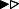
\includegraphics[width=\textwidth]{comparisonOptional.png}
	\caption{Vergleich zwischen einer optionalen und vollwertigen Ein/Ausgabe in KNIME}
	\label{img:comparisonOptional}
\end{figure}

\begin{figure}[H]
	\centering
	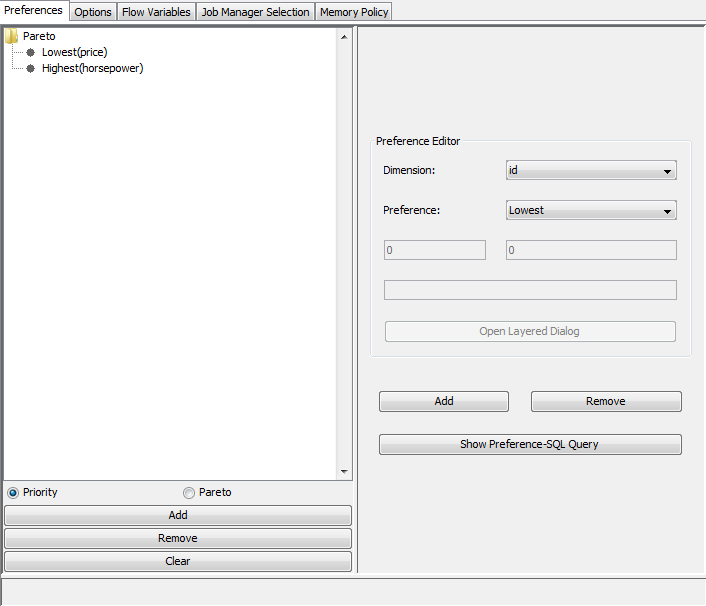
\includegraphics[scale=0.6]{prefCreatorNodeDialog.png}
	\caption{PreferenceEditor, in dem der User seine Präferenzen einstellen kann}
	\label{img:prefCreatorNodeDialog}
\end{figure}

Für die Implementierung des NodeDialogs wurde eine eigene GUI erstellt und keine vorgegebenen Komponenten von KNIME benutzt. 
Im NodeDialog (Figur \ref{img:prefCreatorNodeDialog}) ist auf der linken Seite eine Baumdarstellung zu sehen. Dort können neue Prioritäts oder Pareto Knoten mit dem 'Add' Button hinzugefügt werden. Dabei kann ein Prioritätsknoten nur zu einem leeren Baum oder zu einem Paretoknoten hinzugefügt werden und umgekehrt. Weiterhin können diese Knoten einzeln mit dem 'Remove' Button oder gemeinsam mit dem 'Clear' Button entfernt werden. Mit den beiden Optionen 'Priority' und 'Pareto' kann entschieden werden, welche Knoten gerade bearbeitet werden sollen. Dies führt dazu, dass nur Prioritätsknoten hinzugefügt/entfernt werden können, falls die entsprechende Option ausgewählt ist und vice versa.

Auf der rechten Seite kann der User durch das Selektieren eines Prioritäts oder Pareto Knotens eine Präferenz zu dem selektierten Knoten hinzufügen. Der User hat für die Erstellung einer Präferenz zwei Auswahlboxen. Eine ist für die Auswahl der Dimensionen, die den Spaltennamen des BufferedDataTables gleichen, zuständig. Die andere Box dagegen ermöglicht die Auswahl der Präferenzen für die ausgewählte Dimension. Folgende Präferenzen, deren Prinzip in Kapitel \ref{ch:Grundlagen:sec:präferenzen} genauer erklärt wurden, stehen zur Auswahl: LOWEST, HIGHEST, AROUND, BETWEEN, BOOLEAN und LAYERED. Für die AROUND, BETWEEN und BOOLEAN Präferenzen gibt es Eingabefelder für die Werte, die für diese Präferenzen benötigt werden. Diese Eingabefelder sind je nachdem, was für eine dieser Präferenzen gerade ausgewählt ist, aktiviert oder deaktiviert. Zu beachten ist, dass Dimensionen mit nicht-numerischen Werten nur mit einer LAYERED Präferenz priorisiert werden können. 
Zusätzlich zu allen vorliegenden Dimensionen gibt es eine \enquote{CustomDimension}. Diese Dimension kann der User in einem der Eingabefelder selber erstellen. Es können Dimensionen geteilt werden, falls ein bestimmter Prozentsatz präferiert werden soll. Dies ist vor allem im Sport sinnvoll, da dadurch gelungene Torschüsse in Vergleich zu Torschussversuchen gesetzt werden können. Es können aber auch boolische Präferenzen erstellt werden wie zum Beispiel 'price < 16000'. Der User hat damit freie Auswahl seine eigenen Dimensionen zu erstellen und diese zu präferieren. Die \enquote{CustomDimension} erlaubt alle Präferenzen außer der LAYERED Präferenz, da keine Werte vorhanden sind, da diese erst bei der Abfrage des Queries entstehen. Sie ist auch die einzige Dimension, welche die BOOLEAN Präferenz, erlaubt. 

Für die LAYERED Präferenz kann der User den LayeredDialog öffnen. Das Öffnen dieses Dialogs befähigt den User in einem separatem Fenster die Werte der ausgewählten Dimension nach Wichtigkeit zu sortieren.
Auf der linken Seite des LayeredDialogs kann der User positive Layer oder negative Layer hinzufügen und entfernen. Welche Layer hinzugefügt oder entfernt werden, wird durch die Option 'Negative Layers' bestimmt. Auf der rechten Seite kann der User die ausgewählten Werte zur ausgewählten Layer hinzufügen. Werte in einer positiven Layer werden allen darunterliegende Layern bevorzugt. Wohingegen Werte in einer negativen Layer gemieden werden. In dem vorliegenden Beispielfall (Abbildung \ref{img:prefCreatorLayeredDialog}) sieht die Priorisierung folgendermaßen aus: grün > schwarz > andere Autofarben > rot. 

\begin{figure}[H]
	\centering
	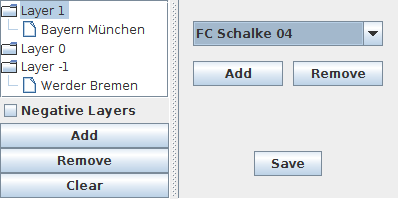
\includegraphics[width=0.7\textwidth]{prefCreatorLayeredDialog.png}
	\caption{LayeredDialog}
	\label{img:prefCreatorLayeredDialog}
\end{figure}

Anschließend wird bei der Ausführung des Nodes, die Nodebaumstruktur des NodeDialogs durchlaufen.
Bei der Generierung des Preference-Querys wird für jeden Prioritätsknoten ein 'PRIOR TO' und für jeden Paretoknoten ein 'AND' zum Query hinzugefügt. Bei der Erreichung einer Basis-Präferenz wird die für diese Präferenz entspreche Preference-SQL Syntax hinzugefügt. Da die CustomDimension noch nicht von Preference-SQL unterstützt wird, kommt es zu keinen Ergebnissen des PreferenceSQL Nodes (siehe Abschnitt \ref{ch:Implementierung:sec:prefSQL}), falls Preference-Queries diese Präferenz enthalten. Die anderen Nodes, die mit dem Score-Query arbeiten, können mit Präferenzen auf dieser Dimension jedoch umgehen. 

Falls beim Durchlaufen des Baumes für die Generierung des Score-Querys eine Basispräferenz erreicht wird, gelten folgende Regeln: Für die LOWEST Präferenz wird nur der Dimensionsname zur Query hinzugefügt. Das selbe gilt für die HIGHEST Präferenz, wofür hier jedoch noch diese mit $-1$ multipliziert wird. Dies hat den Sinn dahinter, dass dadurch alle Scores einheitlich minimiert werden können. Für jede AROUND Präferenz wird $abs(z-v)$, für jede BETWEEN Präferenz $v \in{[low, up]}$ then $0$ else if $v < low$ then $(low - v)$ else $(v - up)$ und für jede BOOLEAN Präferenz $-v$ als Statement zum Query hinzugefügt. In diesen Statements entspricht $v$ dem Dimensionsnamen, $z$ dem vom User eingegebenen Wert für die AROUND Präferenz und $low$ und $up$ für die entsprechenden Intervallgrenzen der BETWEEN Präferenz. 
Für die LAYERED Präferenz wird ein CASE Statement erstellt. Dieses gibt allen Datensätzen, die in der ausgewählten Dimension einen Wert in Layer 1 haben, einen Wert, der der Anzahl an positiven Layers  entspricht. Dieser Ausgabewert wird für jede weitere positive Layer reduziert. Für die erste negative Layer wird der Wert $-1$ vergeben und dieser für jede weitere Layer um $-1$ herunter gezählt. Alle Datensätze die einen Wert in Layer 0 haben, bekommen dementsprechend den Score 0. Zum Schluß wird das CASE Statement mit $-1$ multipliziert, damit auch diese Scores minimiert werden können.
In der Tabelle \ref{tbl:scoreComputation} wird dies an Beispielen genauer verdeutlicht. In der linken Spalte ist die Preference-SQL Syntax der Präferenz zu sehen und in der rechten Spalte das entsprechende Score-Query Statement. 

\begin{table}[H]
  \centering
  \begin{tabular}{|M{4cm}|M{10cm}|}
    \hline
    price LOWEST &  $price$ \\ \hline
    price HIGHEST & $-price$ \\ \hline
    price AROUND 16000 & $abs(16000-price)$ \\ \hline
    price BETWEEN 0,16000 & CASE WHEN price $\geq 0.0$ AND price $\leq 16000.0$ THEN $0$ WHEN price $< 0.0$ THEN ($0.0 - price$) WHEN $price > 16000.0$ THEN ($price-16000.0$) END \\ \hline
    price > 16000 BOOLEAN & price > 16000 \\ \hline
    color LAYERED (('green','black'), OTHERS, ('red')) & -(CASE WHEN color IN ('green', 'black') THEN 1 WHEN color IN ('brown', 'yellow', 'white', 'blue', 'silver') THEN 0 WHEN color IN ('red') THEN -1 END) \\ \hline
  \end{tabular}
  \newline\newline
  \caption{Beispielberechnung der Scores für Basispräferenzen}\label{tbl:scoreComputation}
\end{table}

Für den Präferenzbaum in Figur \ref{img:prefCreatorNodeDialog} werden folgende Queries erzeugt.

\textbf{Preference Query:}
\begin{verbatim}
SELECT * 
FROM (SELECT * FROM car) AS T 
PREFERRING ((price LOWEST PRIOR TO mileage LOWEST) 
AND horsepower HIGHEST)
\end{verbatim}

\textbf{Score Query:}
\begin{verbatim}
SELECT price AS column0,
mileage AS column1,
-(horsepower) AS column2 
FROM (SELECT * FROM car) as T
\end{verbatim}

Wie in vorherigen Abschnitten erwähnt, müssen für die Berechnung einer Skyline Datensätze auf Dominanz getestet werden. Jedoch wird für diese Arbeit nicht mit den orginalen Daten gearbeitet, sondern mit sogenannten Scores. Diese repräsentieren die eingetragenen Präferenzen des Users und sind in der Scoretabelle enthalten. Für die Vergleiche zweier Datensätze wird zusätzlich die Baumstruktur des NodeDialogs benötigt. Damit diese an andere Nodes weitergegeben kann, muss sie in einem bestimmten Format umgewandelt und als Flowvariable weitergegeben werden. 
Für die Erstellung dieses Format wird wieder der Baum durchlaufen. Anfangs wird eine komplexe Präferenz $P_0$ erstellt, die dem Wurzelknoten des Baumes entspricht. In Beispiel aus Abbildung \ref{img:prefCreatorNodeDialog} ist dies der Paretoknoten. Die Art dieser Präferenz wird als erstes vermerkt. Als nächsten Schritt werden die Kinder dieses Knotens durchlaufen. Falls eines der Kinder ein Blatt und damit eine Basispräferenz ist, wird der entsprechende Spaltenname der Scoretabelle vermerkt. Falls es jedoch eine komplexe Präferenz (Prioritäts- oder Paretoknoten) ist, wird diese als nächste komplexe Präferenz vermerkt. Für den Beispielbaum ist einer der Kinder ein Prioritätsknoten und somit eine weitere komplexe Präferenz, die als $P_1$ vermerkt wird. Weiterhin hat der Paretoknoten noch die Basispräferenz horsepower LOWEST. Folglich wird der Spaltenname dieser Präferenz eingetragen. Nun wird dieser Vorgang für jede komplexe Präferenz in $P_0$ wiederholt. Da sowohl $P_0$ als auch $P_1$ keine weiteren komplexen Präferenzen besitzen, endet die Konvertierung des Baumes bei abgeschlossener Formatierung von $P_1$.
Hier ist noch anzumerken, dass falls eine komplexe Präferenz mehr als zwei Kinder besitzt, diese in komplexe Präferenzen unterteilt wird. Für einen Baum mit einem einzelnen Paretoknoten, der drei Basispräferenzen als Kinder besitzt, würden die Flowvariablen wie in Tabelle \ref{tbl:threeChilds} aussehen.

\begin{table}[H]
  \centering
  \begin{tabular}{|M{4cm}|M{10cm}|}
    \hline 
    Flowvariblenschlüssel & Flowvaribleninhalt \\ \hline 
    P0 &  Pareto,P1,column2 \\ \hline
    P1 & Priority,column0,column1\\ \hline
  \end{tabular}
  \newline\newline
  \caption{Flowvariablen der serialisierten Baumstruktur}\label{tbl:serialization}
\end{table} 

\begin{table}[H]
  \centering
  \begin{tabular}{|M{4cm}|M{10cm}|}
    \hline   
    Flowvariblenschlüssel & Flowvaribleninhalt \\ \hline 
    P0 &  Pareto,P1,column2 \\ \hline
    P1 & Pareto,column0,column1\\ \hline
  \end{tabular}
  \newline\newline
  \caption{Die Flowvariablen für einen einzelnen Paretoknoten mit drei Basispräferenzen als Kinder}\label{tbl:threeChilds}
\end{table}

Nach Ausführung des Nodes liegt das in den Node eingehende DatabasePortObject, der optionale BufferedDataTable und die Flowvariablen, die den Score-Query, Preference-Query und die Baumstruktur in einem bestimmten Format enthalten, vor.
Mit diesen Daten kann nun die Skyline berechnet werden.
%% ==============================
\section{PreferenceSQLExtract Node}
\label{ch:Implementierung:sec:prefSQLExtract}
%% ==============================
Dieser Abschnitt befasst sich mit dem PreferenceSQLExtract Node (siehe Abbildung \ref{img:prefSQLExtractorLogo}). Dieser nimmt als Eingabe ein DatabasePortObject, welches von einem PreferenceSQLCreator Node kommen muss, da dieser Node die dazugehörigen FlowVariablen genau genommen einen Preference-Query, benötigt. 
Der Test, ob ein Preference-Query vorliegt wird in der $configure$ Methode des NodeModels vorgenommen. Da jede Flowvariable mit einem entsprechenden Schlüssel gespeichert und geladen wird, besteht die Prüfung nur allein darin, ob dieser Key in der Map der Flowvariablen enthalten ist.  

\begin{figure}[H]
	\centering
	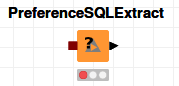
\includegraphics[width=0.25\textwidth]{prefSQLExtractorLogo.png}
	\caption{PreferenceSQLExtract Node}
	\label{img:prefSQLExtractorLogo}
\end{figure}

In der $execute$ Methode wird ein leerer BufferedDataTable mit einer Spalte und einer Reihe erstellt. Dieser einen Zelle wird der Preference-Query hinzugefügt. Der User kann nach erfolgreicher Ausführung des Nodes diesen BufferedDataTable öffnen und den entsprechenden Query kopieren.
%% ==============================
\section{PreferenceSQL Node}
\label{ch:Implementierung:sec:prefSQL}
%% ==============================
\begin{figure}[H]
	\centering
	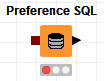
\includegraphics[width=0.22\textwidth]{prefSqlLogo.png}
	\caption{PreferenceSQL Node}
	\label{img:prefSQLLogo}
\end{figure}

Der PreferenceSQL Node (siehe Figur \ref{img:prefSQLLogo}) benötigt als Input ein DatabasePortObject. Da der Preference-Query benötigt wird, erscheint eine Fehlermeldung, falls dieser nicht vorhanden ist. Dies hat zur Folge, dass nur DatabasePortObjects von einem PreferenceCreator Node zulässig sind. 

Bisher ist für diesen Node die Abfrage des Preference-Query nur auf der Postgres-Datenbank des gemini Servers der Universität Augsburg möglich. Jedoch soll in der Zukunft diese Abfrage auf diesen Server weitergeleitet werden, damit auch Abfragen von anderen Datenbanken möglich ist.
Derzeit fragt der Node mit der vorhandenen Datenbankverbindung den Preference-Query ab und liefert die entsprechenden Daten als BufferedDataTable zurück. Dieser wird als Ausgabe zurückgegeben und kann vom Benutzer nach Ausführung des Nodes betrachtet werden.

Im NodeDialog kann der User noch zusätzlich die Anzahl der zurückgegeben Datensätze einschränken. Hierfür wird ein LIMIT Statement an den bisherigen Preference-Query angehängt. Da die eigentliche Ausgabe eine Skyline ist, kann mit dieser Eingabe eine repräsentative Skyline erstellt werden. Jedoch muss bedacht werden, dass die Datensätze zufällig in den BufferedDataTable hinzugefügt werden und somit keine hohe Repräsentationsgüte gewährleistet ist.
%% ==============================
\section{Block-Nested-Loop Node}
\label{ch:Implementierung:sec:bnlNode}
%% ==============================
\begin{figure}[H]
	\centering
	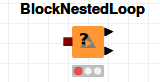
\includegraphics[width=0.22\textwidth]{bnlLogo.png}
	\caption{Block-Nested-Loop Node}
	\label{img:bnlLogo}
\end{figure}

Der Block-Nested-Loop Node benötigt als Eingabe ein DatabasePortObject. In der $configure$ Methode wird geprüft, ob die Flowvariablen einen Score-Query und die konvertierte Baumstruktur enthalten. Falls dies nicht der Fall ist, wird ein Fehler an den User ausgegeben.
Durch die Abfrage des Score-Querys an die Datenbankverbindung kann die Scoretabelle erzeugt werden. Diese Tabelle enthält die Scores der Datensätze, die auf den Präferenzen des Users basieren.

Mithilfe dieser Scores und dem Block-Nested-Loop Algorithmus kann nun die Skyline berechnet werden.
Hierfür wird zuerst der Block-Nested-Loop Algorithmus standardgemäß nach Kapitel \ref{ch:Analyse:sec:skyAlgos:subsec:bnl} ausgeführt. Falls die Dominanz zwischen zwei Datensätzen geprüft werden muss, wird zuerst die konvertierte Baumstruktur durchlaufen. Diese enthält eine Reihe von komplexen Präferenzen.
Wie im vorherigen Abschnitt erwähnt, sieht die Struktur von komplexen Präferenzen folgendermaßen aus: Art der Präferenzverknüpfung, Präferenz 1, Präferenz 2 (siehe Tabelle \ref{tbl:serialization})
Dabei können Präferenz 1 und 2 weitere komplexe Präferenzen sein, die auch durchlaufen werden müssen bis eine komplexe Präferenz gefunden wird, die nur aus Basispräferenzen bzw. den entsprechenden Spaltennamen der Scoretabelle besteht.
Das Durchlaufen wird rekursiv durchgeführt und startet mit einer der im weiteren Verlauf angegebenen Funktionen. Mit welcher gestartet wird hängt von der ersten komplexen Präferenz $P0$ und deren Art von Präferenzverknüpfung ab.
Präferenzverknüpfung können vom Typ 'Priority' oder 'Pareto' sein. Je nach Verknüpfungsart wird eine andere Formel benutzt.

Gegeben seien zwei Datensätze $D_1$ und $D_2$ und zwei Präferenzen $P_1$ und $P_2$.
Es soll geprüft werden, dass Datensatz $D_1$ $D_2$ dominiert: $D_1 <_P D_2$, wobei $P$ eine Verknüpfung der beiden Präferenzen $P_1$ und $P_2$ darstellt.

Die Prüfung der Dominanz hängt somit von der Art der Verknüpfung der Präferenzen ab. Für die Prioritätsverknüpfung werden folgende Formeln benutzt:

\textbf{Priorisierungspräferenz:} $P = P_1$ \& $P_2:$ \\ \\
Dominanz Formel: \\
$D_1 <_P D_2$ iff $D_1 <_{P_1} D_2 \lor (D_1 =_{P_1} D_2 \land D_1 <_{P_2} D_2)$ \\ \\
Gleichwertigkeits Formel: \\
$D_1 =_P D_2$ iff $D_1 =_{P_1} D_2 \land D_1 =_{P_2} D_2$ \\

Falls jedoch die Art der Verknüpfung vom Typ Pareto vorliegt, wird die Dominanz mit folgenden Formeln geprüft:

\textbf{Paretopräferenz:} $P = P_1 \otimes P_2:$ \\ \\
Dominanz Formel:\\
$D_1  <_P D_2$ iff $(D_1 <_{P_1} D_2 \land (D_1 <_{P_2} D_2 \lor D_1 =_{P_2} D_2)) \lor (D_1 <_{P_2} D_2 \land (D_1 <_{P_1} D_2 \lor D_1 =_{P_1} D_2))$ \\ \\
Gleichwertigkeits Formel: \\
$D_1 =_P D_2$ iff $D_1 =_{P_1} D_2 \land D_1 =_{P_2} D_2$ \\

Wie schon im Abschnitt \ref{ch:Implementierung:sec:prefCreatorNode} erwähnt, werden die Scores so bestimmt, dass alle einheitlich minimiert werden können. Das bedeutet, dass falls einer der beiden Präferenzen, $P_1$ oder $P_2$, eine Basispräferenz ist, werden die Scores für diese Präferenz von beiden Datensätzen verglichen. Angenommen $P_2$ ist eine Basispräferenz, dann dominiert $D_1$ $D_2$, falls $D_1$ für diese Präferenz den geringeren Score hat. Dieser Test auf Dominanz für $P_2$ entspricht in den Formeln $<_ {P_2}$. Im Gegensatz dazu, prüft $=_{P_2}$ ob die Werte der beiden Datensätze für diese Präferenz gleich sind. 
Falls jedoch einer der beiden Präferenzen eine komplexe Präferenz ist, muss diese zuerst berechnet werden, indem die entsprechenden Formeln für diese Präferenz angewandt werden. Bei einem Vergleich auf Gleichheit wird die Gleichheitsformeln angewandt und auf den Vergleich auf Priorität die entsprechende Dominanzformel. Ob die Pareto oder Prioritätsformeln benutzt werden, hängt von der Verknüpfungsart der zu betrachtenden komplexen Präferenz ab. Diese Vorgehensweise wird nun an dem Beispiel in Tabelle \ref{tbl:serialization} verdeutlicht.

Als erstes wird $P_0$ betrachtet, da dies der Wurzelknoten des Baumes ist. Diese komplexe Präferenz besitzt die Verknüpfungsart Pareto. Aus diesem Grund wird für die Prüfung auf Dominanz die Dominanzformel für Paretopräferenzen benutzt. Wie zu sehen ist, besteht $P_0$ aus einer komplexen Präferenz $P_1$ (= Präferenz 1) und einer Basispräferenz (= Präferenz 2). Für die Basispräferenz werden die Scores der beiden Datensätze von Spalte column2 verglichen. Für $=_{P_2}$ wird $true$ zurückgegeben, falls die beiden Werte identisch sind. Für $<_{P_2}$ wird $true$ zurückgegeben, falls der Wert von $D_1$ kleiner ist als der von $D_2$.
Bei der komplexen Präferenz werden statt den Vergleichen die entsprechenden Formeln aufgerufen und mit deren Rückgabewerte weitergearbeitet. Hierbei muss noch  beachtet werden, dass hierfür nicht mehr die Verknüpfungsart von $P_0$ betrachtet wird, sondern die von $P_1$. Deshalb wird für $=_{P_1}$ die Gleichwertigkeitsformel und für $<_{P_1}$ die Dominanzformel für Prioritätspräferenzen aufgerufen. 
Da nun alle Werte für alle Vergleiche für die Dominanzformel von $P_0$ vorliegen und keine weiteren komplexen Präferenzen vorhanden sind, kann das Ergebnis bestimmt werden. Das Ergebnis dieser Formel liefert $true$ zurück, wenn $D_1$ $D_2$ dominiert.

Der Block-Nested-Loop Algorithmus läuft ganz normal durch bis alle undominierten Datensätze der Scoretabelle gefunden sind. Der Node kann dann anhand der RowIDs dieser undominierten Datensätze die undominierten Datensätze der Originaltabelle ausgeben, da diese die gleichen RowIDs besitzen.

Der NodeDialog erlaubt es dem Benutzer für den Block-Nested-Loop Algorithmus eine Größe für das Fenster $w$ zu bestimmen. Weitere Eingaben für diesen Node sind nicht nötig, da die meisten Einstellungen durch Flowvariablen des PreferenceCreator Nodes schon vorhanden sind.

Der Block-Nested-Loop ermöglicht auch eine Darstellung der Datensätze mittels eines NodeViews. In Abbildung \ref{img:bnlSkyline} kann eine Skyline des Autodatensatzes für die Präferenzen in Figur \ref{img:prefCreatorNodeDialog} betrachtet werden.

\begin{figure}[H]
	\centering
	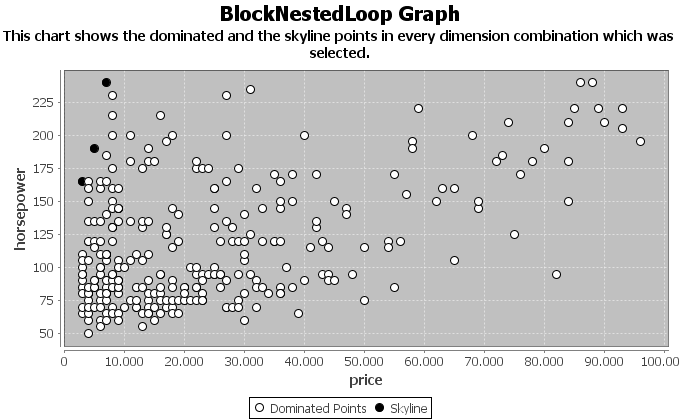
\includegraphics[width=0.9\textwidth]{bnlSkyline.png}
	\caption{Skyline-Datensätze, die durch die Block-Nested-Loop Node entsteht}
	\label{img:bnlSkyline}
\end{figure}
%% ==============================
\section{DominationMaximizer Node}
\label{ch:Implementierung:sec:dominationMaximizerNode}
%% ==============================
\begin{figure}[H]
	\centering
	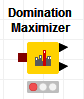
\includegraphics[width=0.26\textwidth]{domMaximizerLogo.png}
	\caption{DominationMaximizer Node}
	\label{img:domMaximierLogo}
\end{figure}

Der DominationMaximizer Node berechnet die repräsentative Skyline und benötigt dafür keine Skyline wie die meisten anderen repräsentativen Skylinealgorithmen. Die Eingabe ist hier wieder das DatabasePortObject eines PreferenceCreator Nodes, da dieser Node auch wieder die Präferenzen des Users mithilfe der Scoretabelle berücksichtigt. 

Die erste Ausgabe besteht aus den $k$ Skylinedatensätzen, die zusammen die Anzahl der dominierten Datensätze maximieren. Die zweite Ausgabe ist die Skyline $S_P$, die während der Durchführung des Algorithmus berechnet wird. Mit diesen beiden Ausgaben kann mithilfe des Nodes in Abschnitt \ref{ch:Implementierung:sec:skyVisualizer} ein Graph erstellt werden. 

Der einzige Zweck des NodeDialogs besteht darin die Größe der repräsentativen Skyline mit einem Parameter $k$ festzulegen. Für eine schnelle Ausführung des Nodes wird wie bei jedem anderen Node für die Eingabeparameter ein Standardwert festgelegt. Somit kann der User den Node nach Erstellung ausführen ohne jemals den NodeDialog geöffnet zu haben.  

Der in der $execute$ Methode auszuführender Algorithmus für diesen Node wurde in Kapitel \ref{ch:Analyse:sec:repSkyAlgos:subsec:domMax} vorgestellt. 
%% ==============================
\section{DistanceBasedResolver Node}
\label{ch:Implementierung:sec:distBasedResolverNode}
%% ==============================
\begin{figure}[H]
	\centering
	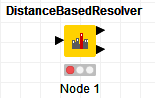
\includegraphics[width=0.26\textwidth]{distBasedResolverLogo.png}
	\caption{E-Greedy Node}
	\label{img:distBasedResolverLogo}
\end{figure}

Der DistanceBasedResolver Node benötigt als Eingabe einen BufferedDataTable, der nur Datensätze, die sich gegenseitig nicht dominieren, besitzt und somit einer Skyline entspricht. Der Node kann jedoch mit jeden beliebigen BufferedDataTable ausgeführt werden. Dies hat jedoch zur Folge, dass die Ausgabe meistens keiner repräsentativen Skyline entspricht. In der $configure$ Methode wird geprüft, ob Flowvariablen eines PreferenceCreator Nodes vorhanden sind. Dies hat zur Folge, dass ein PreferenceCreator Node im Datenfluss existieren muss.

Wie schon in Kapitel \ref{ch:Analyse:sec:repSkyAlgos:subsec:disBasedRepSky} erwähnt, werden die Datensätze für die repräsentative Skyline gewählt, die als Mittelpunkte von Kreisen dienen. Diese Kreise sollten einen geringen Radius besitzen und so viele Datensätze wie möglich umfassen.  

Der erste Output entspricht dieser repräsentativen Skyline und enthält somit alle Datensätze, die vom Algorithmus zurückgegeben werden. Der zweite Output ist der BufferedDataTable, der als Input in den Node hinein kommt und dient als Input für den Node in Abschnitt \ref{ch:Implementierung:sec:skyVisualizer}.

Der NodeDialog bietet dem User ein Eingabefenster, um die Anzahl der repräsentativen Skylinedatensätze, die ausgegeben werden, zu bestimmen. Falls diese Zahl höher oder gleich der Anzahl der Datensätze des Inputs ist, werden alle Datensätze ausgegeben.
%% ==============================
\section{E-Greedy Node}
\label{ch:Implementierung:sec:eGreedyNode}
%% ==============================
\begin{figure}[H]
	\centering
	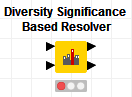
\includegraphics[width=0.26\textwidth]{eGreedyLogo.png}
	\caption{E-Greedy Node}
	\label{img:eGreedyLogo}
\end{figure}

Dieser Node implementiert den Algorithmus aus Kapitel \ref{ch:Analyse:sec:repSkyAlgos:subsec:eGreedy} und benötigt daher als Eingabe eine Skyline. Aus dieser werden aufgrund von Diversität und Signifikanz die $k$ besten Datensätzen ausgegeben.

Die Anzahl der repräsentativen Skyline Datensätze, die ausgegeben werden sollen, kann der Benutzer im NodeDialog einstellen. Zusätzlich kann der Diversitäts- und Signifikanzfaktor dort eingestellt werden. Der Diversitätsfaktor steht für $\lambda$ und der Signifikanzfaktor für $1-\lambda$. Bei Eingabe einer dieser Parameter, wird der andere dementsprechend angepasst, sodass die Summe beider Werte immer $1$ ergibt.
Für die Berechnung der Signifikanz wird eine Sigmoidfunktion benutzt, da diese Thresholds des Benutzers berücksichtigen kann. Somit kann der User im NodeDialog für jede Dimension entscheiden, ob er einen einzelnen Threshold, einen Intervallthreshold oder gar keinen eingeben möchte. (siehe Figur \ref{img:eGreedyNodeDialog}) Falls der User vor der Ausführung des Nodes niemals den NodeDialog geöffnet und keine Thresholds angegeben hat, werden alle Datensätze als gleich signifikant angesehen und somit wird nur Diversität berücksichtigt. 

\begin{figure}[H]
	\centering
	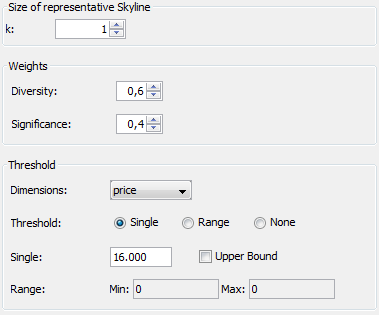
\includegraphics[width=0.8\textwidth]{eGreedyNodeDialog.png}
	\caption{NodeDialog des E-Greedy Nodes}
	\label{img:eGreedyNodeDialog}
\end{figure}

Nach Ausführung des Algorithmus werden zwei Outputs ausgegeben. Die $k$ repräsentativen Skylinedatensätze und die ursprüngliche Skyline. Für die Skyline aus Figur \ref{img:bnlSkyline} und der Eingaben im NodeDialog ergibt sich die repräsentative Skyline, die in Abbildung \ref{img:eGreedyOutput} zu sehen ist.

\begin{figure}[H]
	\centering
	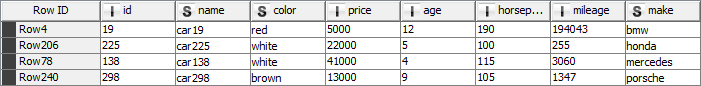
\includegraphics[width=0.8\textwidth]{eGreedyOutput.png}
	\caption{Repräsentative Skyline, die durch den E-Greedy Node entsteht}
	\label{img:eGreedyOutput}
\end{figure}
%% ==============================
\section{SkylineVisualizer Node}
\label{ch:Implementierung:sec:skyVisualizer}
%% ==============================
\begin{figure}[H]
	\centering
	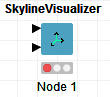
\includegraphics[width=0.26\textwidth]{skyVisualizerLogo.png}
	\caption{Sky Visualizer Node}
	\label{img:skyVisualizerLogo}
\end{figure}

Der Skyline Visualizer Node ist dafür zuständig zwei BufferedDataTable als Eingabe zu nehmen und diese Daten graphisch in einem Koordinatensystem darzustellen. Ein PreferenceCreator Node im Datenfluss wird benötigt, da alle Dimensionen der Originaltabelle erforderlich sind. Für das Koordinatensystem werden nur numerische Dimensionen betrachtet. Außerdem können für weniger als zwei und mehr als drei Dimensionen keine Graphen erstellt werden.

Im NodeDialog (siehe \ref{img:skyVisualizerNodeDialog}) kann der User einstellen wie er seinen Graph beschriftet haben möchte. Zur Auswahl stehen die Beschriftung für einen repräsentativen Skyline Graphen (weiße Punkte: Skyline, schwarz: repräsentative Skyline) oder einen Skyline Graphen(weiß: alle Punkte, die dominiert werden, schwarz: Skyline). Falls dem User keiner dieser Einstellungen zusagt, kann er die Überschrift und die Beschreibung des Graphen auch selbst in Eingabefeldern des NodeDialogs eintragen.

\begin{figure}[H]
	\centering
	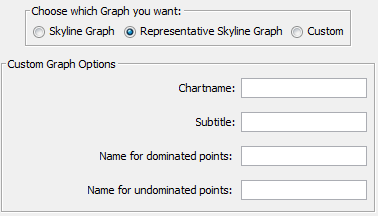
\includegraphics[width=0.8\textwidth]{skyVisualizerNodeDialog.png}
	\caption{NodeDialog des SkylineVisualizer Nodes}
	\label{img:skyVisualizerNodeDialog}
\end{figure}

Für das Autobeispiel in \ref{img:prefCreatorNodeDialog}, welches drei Dimensionen berücksichtigt ergibt sich der Graph in Abbildung. \ref{img:skyVisiualizerView1}. Hierfür wurden drei Graphen für jede mögliche Kombination der Dimensionen erstellt. Um Übersichtlichkeit zu bewahren, gibt es keine Graphen mehr, falls vier oder mehr Dimensionen betrachtet werden sollen.

\begin{figure}[ht]
	\centering
	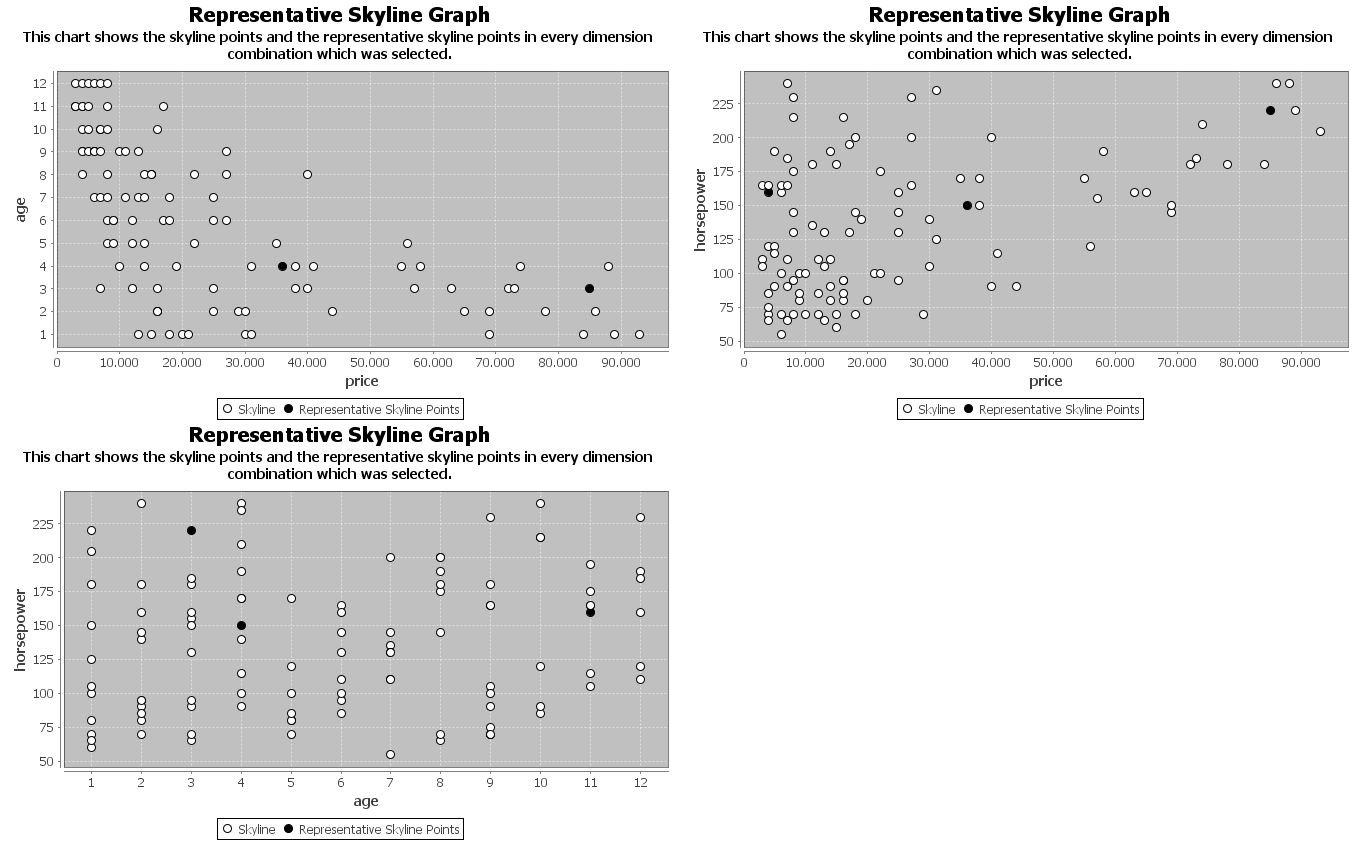
\includegraphics[width=0.8\textwidth]{skyVisualizerView2.png}
	\caption{View des Skyline Visualizer Nodes für drei Dimensionen}
	\label{img:skyVisiualizerView2}
\end{figure}

Falls für das Beispiel der Prioritätsknoten wegfällt und es auf die zwei Präferenzen 'price LOWEST' und 'horsepower' HIGHEST reduziert wird

\begin{figure}[ht]
	\centering
	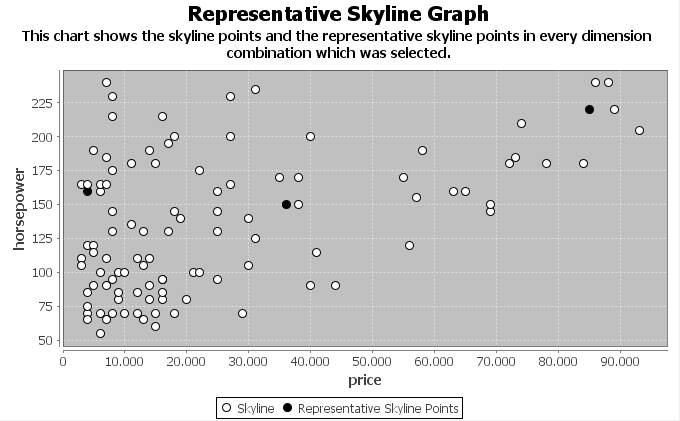
\includegraphics[width=0.8\textwidth]{skyVisualizerView1.png}
	\caption{View des Skyline Visualizer Nodes für zwei Dimensionen}
	\label{img:skyVisiualizerView1}
\end{figure}
%% ==============================
%%% End: 